
\section{Introduction}

In this chapter we evaluate the performance of linear correlation methods based on
eigen-analysis when applied to the related problems of image retrieval and image
annotation. In both problems, we have a corpus of images with corresponding text captions
or text keywords. We may also have a text document or article associated with each
image-caption pair.  Image retrieval allows a user to enter a text query to retrieve
relevant images from the corpus. Automatic image annotation allows a user to enter an
image as a query to retrieve relevant keywords about that image. These interrelated
machine learning problems require a way of transforming both words and images into objects
that are understandable by machines \cite{smeulders2000content}. For such problems, we
naturally assume that the words in a caption are correlated with features of the image and
also representative of the (possibly) associated text document. Therefore, correlation
detection algorithms are natural candidates to help solve these problems. Using regression
techniques relying on these correlated components, we can predict relevant image features given a
set of words. Similarly, given a set of image features, we can predict relevant keywords.

Canonical Correlation Analysis (CCA) is a dimensionality reduction algorithm for two
datasets. For each dataset, CCA learns a linear transformation such that the transformed
datasets are maximally correlated. Representing data in a lower-dimensional, maximally
correlated space allows learning algorithms to more easily and more efficiently exploit
such naturally existing correlations. Image retrieval and image annotation are natural
applications for CCA as there are exactly two datasets, images (or text documents) and
text captions, that are assumed to have correlated features.

CCA and various modifications have been previously applied to information retrieval
problems. In \cite{chaudhuri2009multi}, the authors use CCA to cluster Wikipedia articles
based on their text and incoming and outgoing links. In \cite{hardoon2004canonical}, the
authors implemented a CCA based image retrieval system on a limited set of image types
(sports, aviation, and paintball). The authors in \cite{hardoon2006correlation} used a
kernel version of CCA for automatic image annotation on a more varied set of images. 

While these papers report moderate performance when using CCA for information retrieval
tasks, CCA is fundamentally flawed. When the number of image-caption pairs is less
than the combined dimension of the textual and image features, CCA returns random linear
transformations and a perfect correlation between datasets
\cite{pezeshki2004empirical}. For this reason, CCA is often overlooked when considering
appropriate algorithms for machine learning problems. However, as was shown in Chapter 4
in this thesis, Informative CCA (ICCA) overcomes the massive performance loss of
CCA in the low-sample regime. By applying insights from random matrix theory to eliminate
noisy subspaces, ICCA can detect correlations in the low-sample low-SNR regime where CCA
would otherwise fail to do so. 

The purpose of this chapter is to showcase that intelligent correlation algorithms are
indeed worthy of further investigation by the information retrieval community. In Section
\ref{sec:cca}, we provide a brief overview of CCA and ICCA including their mathematical
formulations and solutions. In Section \ref{sec:propose}, we outline how to use linear
correlation algorithms for image retrieval and automatic image annotation. For captions
and articles/documents, we create feature vectors using tf-idf weightings. For images, we
construct visual word feature vectors based on SIFT features. We describe how to train a
correlation model on a corpus and how to use the model to predict one modality from the
other. In Section \ref{sec:results}, we apply our image retrieval and annotation system on
four datasets. First, we visually compare the performance of CCA and ICCA based image
retrieval and image annotation on the Pascal dataset. Second, we specifically consider the
image annotation problem on the University of Washington Ground Truth dataset, the Gold
Standard Web dataset, and the BBC News dataset. These datasets allow us to compare the
performance of eigen-based correlation algorithms to standard NLP and IR techniques on
three datasets of varying difficulties. We provide a discussion of the benefits and
limitations of eigen-based correlation algorithms in Section \ref{sec:disc} and concluding
remarks in Section \ref{sec:conc}.

\section{Correlation Methods}\label{sec:cca}

Canonical correlation analysis (CCA) is a popular algorithm to identify features of
maximal correlation between exactly two multi-modal datasets. CCA is a dimensionality
reduction algorithm that finds a linear transformation for each dataset such that the
correlation between the two transformed feature sets is maximized
\cite{hotelling1936relations}. These linear transformations are easily found by solving a
quadratic optimization problem; this solution is a closed form expression relying on the
singular value decomposition (SVD) of a matrix product involving the covariance matrices
of each dataset and the cross-covariance matrix between the two datasets. As these covariance
matrices are rarely known \textit{a priori}, practical uses of CCA rely on substituting
sample covariance matrices formed from training data; we call this algorithm empirical CCA.

While we will apply CCA to image retrieval and annotation, CCA is commonly used in a
variety of other disciplines. In \cite{hardoon2004canonical}, CCA is used to learn
semantics of multimedia content by fusing image and text data. CCA is applied to to the
common communications problem of blind equalization of single-input multiple-output (SIMO)
channels in \cite{via2005canonical}. In the field of medical imaging, CCA is used to
determine interactions, or connectivities, between brain areas in fMRI data
\cite{deleus2011functional} and used to fuse fMRI, sMRI, and EEG data
\cite{correa2010canonical}. CCA has also been applied to clustering speakers given an
audio-video dataset \cite{chaudhuri2009multi}. In the more abstract problems of
Gauss-Gauss detection and estimation, \cite{pezeshki2006canonical} shows that standard
detectors and estimators can be written in terms of the solution to CCA.


\subsection{Mathematical Formulation of CCA}\label{sec:cca_form}
Assume that observations $\yI\in\reals^{d_x\times 1}$, $\yII\in\reals^{d_y\times 1}$
are drawn from two distributions $\yI\sim\mathcal{X}$,
$\yII\sim\mathcal{Y}$. Furthermore, assume that the distributions have zero mean,
\textit{i.e.} $\E{\yI}=\E{\yII}=0$. We will use the following notation for the covariance
matrices of the distributions: $\E{\yI\yI^T}=\RI$, $\E{\yII\yII^T}=\RII$,
$\E{\yI\yII^T}=\RIII$.

The goal of CCA is to find a linear transformation for each dataset that maximizes the
correlation between the datasets in the projected spaces. We represent the linear
transformations with the canonical vectors $\xI\in\reals^{d_x\times 1}$ and
$\xII\in\complex^{d_y\times 1}$ and the projection with the canonical variates $\wI=\xI^T\yI$ and
$\wII=\xII^T\yII$. The objective is to find the canonical vectors $\xI$ and $\xII$ that
maximize the correlation between the canonical variates $\wI$ and $\wII$. Formally, the
optimization problem is
\begin{equation}\label{eq:chpt9:cca_opt}
  \begin{aligned}
    &\argmax_{\xI,\xII}&&\rho = \E{\wI\wII}\\
    & \text{subject to}&&\E{\wI^2}=1, \E{\wII^2}=1.
  \end{aligned}
\end{equation}
Substituting the expressions for the canonical variates and the correlation matrices, this
optimization problem may be written as
\begin{equation}\label{eq:chpt9:cca_opt2}
  \begin{aligned}
    &\argmax_{\xI,\xII}&&\rho = \xI^T\RIII\xII\\
    & \text{subject to}&&\xI^T\RI\xI=1, \xII^T\RII\xII=1.
  \end{aligned}
\end{equation}

Standard Lagrange multiplier techniques can be used to solve (\ref{eq:chpt9:cca_opt2}). The
proof is omitted here but please reference
\cite{nielsen2002multiset,nadakuditi2011fundamental,welling2005kcca,kettenring1971canonical,nielsen1994analysis}
if interested. The solution is the following eigenvalue system
\begin{equation}\label{eq:chpt9:cca_eigval_sys}
  \RI^{-1}\RIII\RII^{-1}\RIII^T\,\xI = \rho^2\xI
\end{equation}
with the relationship
\beq\label{eq:chpt9:x2}
\xII=\frac{1}{\rho}\RII^{-1}\RIII^T\,\xI.
\eeq

Solving (\ref{eq:chpt9:cca_eigval_sys}) for the eigenvector corresponding to the largest
eigenvalue solves (\ref{eq:chpt9:cca_opt2}). Substituting this eigenvalue/eigenvector pair in
(\ref{eq:chpt9:x2}) gives the complete solution $\left(\xI,\xII,\rho\right)$ for the transformations
  and maximum correlation between the datasets. Multiple canonical basis vectors may be
  found by recursively finding the next largest eigenvalue and corresponding eigenvector
  in (\ref{eq:chpt9:cca_eigval_sys}). In many learning applications, it is common to project
  onto multiple canonical basis vectors.

 Using a similarity transform, we can frame the eigen-system in (\ref{eq:chpt9:cca_eigval_sys})
 as an SVD problem. Define $f = \RI^{1/2}\xI$ and $g=\RII^{1/2}\xII$. Then
 (\ref{eq:chpt9:cca_eigval_sys}) may be rewritten as
\begin{equation}\label{eq:chpt9:eigval_sys2}
  \RI^{-1/2}\RIII\RII^{-1}\RIII^T\RI^{-T/2}f = \rho^2f.
\end{equation}
Defining $C=\RI^{-1/2}\RIII\RII^{-T/2}$, (\ref{eq:chpt9:eigval_sys2}) can be rewritten as
\begin{equation}\label{eq:chpt9:cca_C_eigval}
  CC^Tf=\rho^2f.
\end{equation}

Clearly, from (\ref{eq:chpt9:cca_C_eigval}), we may obtain a closed form solution for $f$, $g$, and
$\rho$ through the SVD of $C$. Let $FKG^T$ be the SVD of $C$ where
$F=[f_1,\dots,f_{d_x}]$, $K\in\complex^{d_x\times
  d_y}=\diag(k_1,\dots,k_{\min\left(d_x,d_y\right)})$, and $G=[g_1,\dots,g_{d_y}]$. Then the solution
for the canonical vector pair corresponding to the largest canonical correlation is
\beq\label{eq:chpt9:cca_svd_sol}\ba
&\rho = k_1\\
&\xI = \RI^{-1/2}f_1\\
&\xII = \RII^{-1/2}g_1\\
\ea\eeq
with successive pairs of canonical vectors obtained from successive singular vectors and
singular value pairs.

\subsection{Empirical CCA}\label{sec:emp_cca}

The above derivation assumes that the covariance matrices $\RI$, $\RII$, and $\RIII$ are all
known. However, in most applications these covariance matrices are unknown and must be
estimated from data. In such an empirical setting, we assume that we are given $n$
observations, or samples, from each dataset $\yI^{(i)}$ and $\yII^{(i)}$ for
$i=1,\dots,n$ such that $\yI^{(i)}$ and $\yII^{(i)}$ each represent the same object. In
the application for this chapter, $\yI^{(i)}$ will be a text caption and $\yII^{(i)}$
will be the corresponding image or article features. We may stack these observations in
training data 
matrices
\be
X=\left[\yI^{(1)},\dots,\yI^{(n)}\right], \text{ and } 
Y=\left[\yII^{(1)},\dots,\yII^{(n)}\right]
\ee
and use these training data matrices to estimate the unknown covariance matrices via
\beq\label{eq:chpt9:scm}\ba
&\RIhat = \frac{1}{n} XX^T\\
&\RIIhat = \frac{1}{n} YY^T\\
&\RIIIhat = \frac{1}{n} XY^T.\\
\ea\eeq
We may then substitute these covariance matrix estimates in the expression for $C$,
resulting in the estimator
\beq\label{eq:chpt9:cca_Chat}
\widehat{C} = \RIhat^{-1/2}\RIIIhat\RIIhat^{-1/2}.
\eeq
Defining $\widehat{C} =\widehat{F}\widehat{K}\widehat{G}^T$ as the SVD of $\widehat{C}$,
the solution to empirical CCA is
\beq\label{eq:chpt9:cca_svd_sol}\ba
&\widehat{\rho} = \widehat{k}_1\\
&\xIhat = \RIhat^{-1/2}\,\widehat{f}_1\\
&\xIIhat = \RIIhat^{-1/2}\,\widehat{g}_1.\\
\ea\eeq

\subsection{Informative CCA}

A main drawback to CCA is that when then number of samples is less than the combined
dimension of the two datasets ($n<d_x+d_y$), CCA always reports a perfect correlation, no
matter how correlated the datasets actually are \cite{pezeshki2004empirical}. 

In earlier chapters, we demonstrated that informative CCA (ICCA) avoids this drastic performance
loss associated with CCA. Assuming a linear signal-plus-noise model, ICCA uses random
matrix theory insights to trim data SVDs to only include informative subspaces. Formally,
let $U_x\Sigma_xV_x^T$ be the SVD of $X$ and $U_y\Sigma_yV_y^T$ be the SVD of $Y$. Define 
\be\ba
& \widetilde{U}_x = U_x(:,1:k_x) && \widetilde{V}_x = V_x(:,1:k_x)\\
& \widetilde{U}_y = U_y(:,1:k_y) && \widetilde{V}_y = V_y(:,1:k_y)\\
\ea\ee 
where $k_x$ and $k_y$ are the number of informative components in the first and
second datasets, respectively. These may be estimated using standard random matrix theory
principles, as we proposed in earlier chapters. Using these trimmed data matrices, we form
the matrix used for ICCA, 
\beq\label{eq:chpt9:icca_chat} \widetilde{C} =
\widetilde{U}_x\widetilde{V}_x^T\widetilde{V}_y\widetilde{U}_y^T.  \eeq Let $\widetilde{C}
= \widetilde{F}\widetilde{K}\widetilde{G}^H$ be the SVD of this matrix. ICCA returns the
following informative correlation estimate and canonical vectors
\begin{equation}\label{eq:chpt9:icca_rho}
\ba
&\widetilde{\rho} &&= \widetilde{k}_1\\
&\widetilde{x}_1 &&= \RIhat^{-1/2}\widetilde{f}_1\\
&\widetilde{x}_2 &&= \RIIhat^{-1/2}\widetilde{g}_1.\\
\ea
\end{equation}
As we theoretically showed in earlier chapters, ICCA is able to detect correlations in the
low-sample and low-SNR regimes where CCA would not. In these regimes, the linear
transformations that CCA returns are random and contain no information, while the linear
transformations returned by ICCA contain information. With these observations, ICCA may
return meaningful results in image retrieval and annotation where CCA was previously
ignored due to random performance.

\section{System Implementation}\label{sec:propose}

In this section we describe how to use CCA and ICCA for content based image retrieval and
automatic image annotation. A common training stage learns the correlation model necessary
to perform both tasks. Figure \ref{fig:chpt9:training} outlines the training phase when the two
datasets are captions and associated images. Figure \ref{fig:chpt9:training_tt} outlines the
training phase when the two datasets are captions and associated text documents. Each
block is a sub-task that will be described in more detail below. Depending on our dataset,
one pipeline will be more appropriate. For example, the University of Washington Ground
Truth dataset only has images and captions so we will use the pipeline in Figure
\ref{fig:chpt9:training}. However, in the Gold Standard Web dataset, we have access to captions,
images, and associated documents. For this dataset, we only have a few samples of a large
variety of images and so we will used the pipeline in Figure \ref{fig:chpt9:training_tt}. The
output of both pipelines are canonical bases $W_x$ and $W_y$ and the corresponding
canonical correlations, $P$. After training, we may use the correlation model to retrieve
images, which is outlined in Figure \ref{fig:chpt9:test1}, or annotate images, which is outlined
in Figure \ref{fig:chpt9:test2}. These sub-tasks will also be described below.

\begin{figure}[th!]
  \begin{center}
    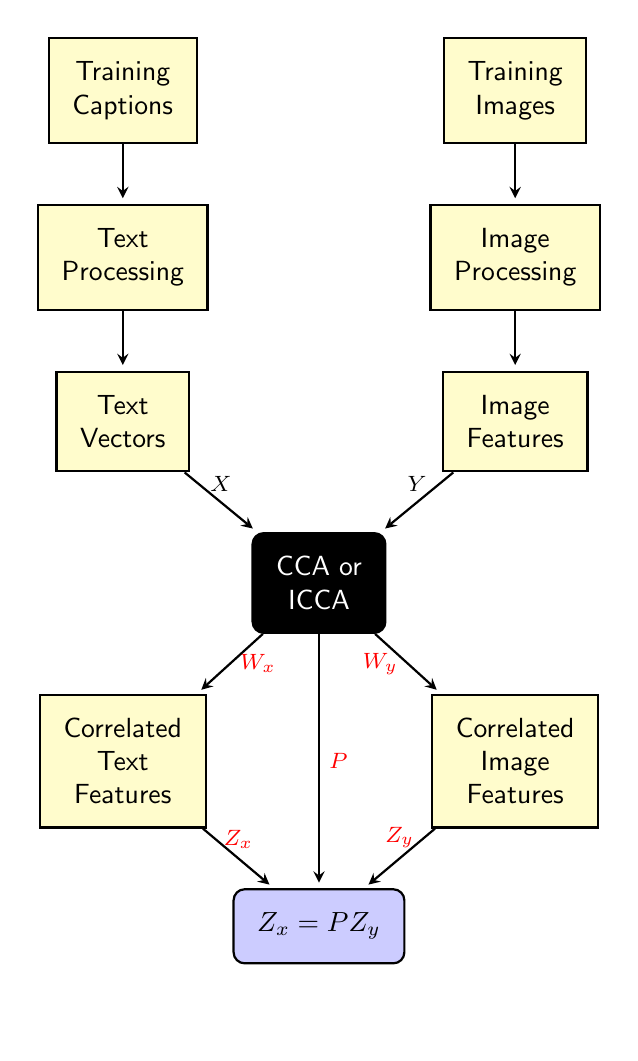
\begin{tikzpicture}[
      font=\sffamily,
      every matrix/.style={ampersand replacement=\&,column sep=2ex,row sep=5ex},
      dataset/.style={draw,thick,fill=yellow!20,inner sep=.3cm},
      sink/.style={dataset,rounded corners,fill=black, text=white},
      app/.style={dataset,rounded corners,fill=blue!20},
      dots/.style={gray,scale=2},
      to/.style={->,>=stealth,shorten >=2pt,thick,font=\sffamily\footnotesize},
      every node/.style={align=center}]

      \matrix{       
        \node[dataset] (cap) {Training \\Captions};
        \&;
        \&\node[dataset] (im) {Training \\ Images};\\

        \node[dataset] (textp) {Text \\ Processing};
        \&;
        \& \node[dataset] (imp) {Image \\Processing};\\


        \node[dataset] (dataset1) {Text \\Vectors};
        \&;
        \& \node[dataset] (dataset2) {Image \\Features};\\

        ;
        \& \node[sink] (blackbox) {CCA or\\ ICCA}; 
        \&; \\

        \node[dataset] (dataset3) {Correlated \\Text \\Features};
        \&; 
        \& \node[dataset] (dataset4) {Correlated\\ Image\\ Features};\\

        ;
        \& \node[app] (application) {$Z_x=PZ_y$};\\
        \&;\\       
      };

      \draw[to] (cap) -- (textp)node[midway,left] {};
      \draw[to] (im) -- (imp)node[midway,right] {};
      \draw[to] (textp) -- (dataset1)node[midway,left] {};
      \draw[to] (imp) -- (dataset2)node[midway,right] {};
      \draw[to] (dataset1) -- (blackbox)node[midway,above] {$X$};
      \draw[to] (dataset2) -- (blackbox)node[midway,above] {$Y$};
      \draw[to] (blackbox) -- (dataset3) node[midway,right] {\textcolor{red}{$W_x$}};
      \draw[to] (blackbox) -- (dataset4) node[midway,left] {\textcolor{red}{$W_y$}};
      \draw[to] (blackbox) -- (application) node[midway,right] {\textcolor{red}{$P$}};
      \draw[to] (dataset3) -- (application) node[midway,above] {\textcolor{red}{$Z_x$}};
      \draw[to] (dataset4) -- (application) node[midway,above] {\textcolor{red}{$Z_y$}};

    \end{tikzpicture}
    \caption{Shared training pipeline for image retrieval and annotation when using raw
      images as the second dataset. The system takes training images and captions as
      inputs and returns the canonical bases $W_x$ and $W_y$ and the correlation
      coefficients $P$.}
    \label{fig:chpt9:training}  
  \end{center}
\end{figure}

\begin{figure}[th!]
  \begin{center}
    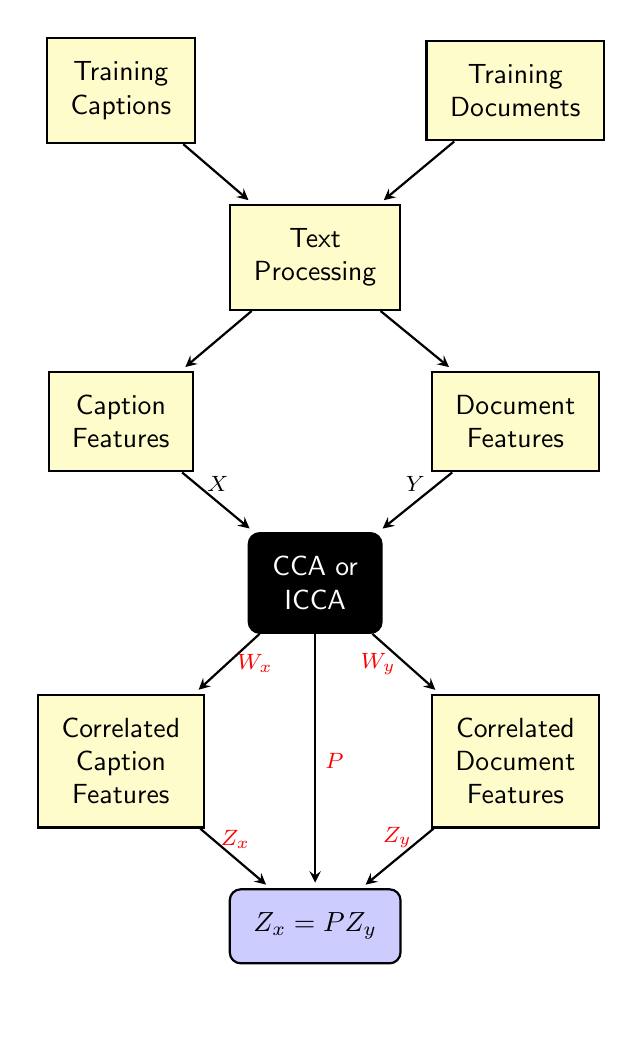
\begin{tikzpicture}[
      font=\sffamily,
      every matrix/.style={ampersand replacement=\&,column sep=2ex,row sep=5ex},
      dataset/.style={draw,thick,fill=yellow!20,inner sep=.3cm},
      sink/.style={dataset,rounded corners,fill=black, text=white},
      app/.style={dataset,rounded corners,fill=blue!20},
      dots/.style={gray,scale=2},
      to/.style={->,>=stealth,shorten >=2pt,thick,font=\sffamily\footnotesize},
      every node/.style={align=center}]

      \matrix{       
        \node[dataset] (cap) {Training \\Captions};
        \&;
        \&\node[dataset] (im) {Training \\ Documents};\\

        ;
        \&\node[dataset] (textp) {Text \\ Processing};
        \&;\\

        \node[dataset] (dataset1) {Caption \\ Features};
        \&;
        \& \node[dataset] (dataset2) {Document \\Features};\\

        ;
        \& \node[sink] (blackbox) {CCA or\\ ICCA}; 
        \&; \\

        \node[dataset] (dataset3) {Correlated \\Caption\\Features};
        \&; 
        \& \node[dataset] (dataset4) {Correlated\\ Document\\ Features};\\

        ;
        \& \node[app] (application) {$Z_x=PZ_y$};\\
        \&;\\       
      };

      \draw[to] (cap) -- (textp)node[midway,left] {};
      \draw[to] (im) -- (textp)node[midway,right] {};
      \draw[to] (textp) -- (dataset1)node[midway,left] {};
      \draw[to] (textp) -- (dataset2)node[midway,left] {};
      \draw[to] (dataset1) -- (blackbox)node[midway,above] {$X$};
      \draw[to] (dataset2) -- (blackbox)node[midway,above] {$Y$};
      \draw[to] (blackbox) -- (dataset3) node[midway,right] {\textcolor{red}{$W_x$}};
      \draw[to] (blackbox) -- (dataset4) node[midway,left] {\textcolor{red}{$W_y$}};
      \draw[to] (blackbox) -- (application) node[midway,right] {\textcolor{red}{$P$}};
      \draw[to] (dataset3) -- (application) node[midway,above] {\textcolor{red}{$Z_x$}};
      \draw[to] (dataset4) -- (application) node[midway,above] {\textcolor{red}{$Z_y$}};

    \end{tikzpicture}
    \caption{Shared training pipeline for image retrieval and annotation when the second
      dataset is associated text documents. The system takes an training captions and
      associated documents as inputs and returns the canonical bases $W_x$ and $W_y$ and
      the correlation coefficients $P$.}
  \label{fig:chpt9:training_tt}  
\end{center}
\end{figure}

\subsection{Text Processing}

Both training pipelines form feature vectors from text (either captions or documents). To
transform text into a machine understandable object, we create a feature vector whose
length is the size of the vocabulary of the training data and whose entries are tf-idf
weights. Once these vectors are created for each caption, we have a caption dataset,
$X\in\reals^{d_x\times n}$ where $d_x$ is the size of the vocabulary and $n$ is the number
of training captions associated with images. Each vector is then normalized to have an
$\ell_2$ norm of 1, so as not to penalize shorter documents. With this type of processing,
feature vector entries represent the importance that the corresponding word
carries in the document. When processing a text query for image retrieval, the text query
is transformed into a $d_x\times 1$ vector using the same tf-idf weighted scheme used to
generate the training dataset. When generating the vocabulary, we used stopword removal
and Porter stemming \footnote{http://tartarus.org/~martin/PorterStemmer/python.txt}.

\subsection{Image Processing}

The training system in Figure \ref{fig:chpt9:training} takes an image database as its second
input. To transform an image into a machine understandable object, we propose to use
visual words, which is an extension of the vector space model for text documents to
images. Here, a feature vector for an image has entries corresponding to the total
occurrences of a ``visual word'' in that image. Each visual word is a cluster of image
features extracted across all training data \cite{yang2007evaluating}. For our
implementation, we use SIFT image features vectors as the feature vectors to cluster.

The Scale Invariant Feature Transform (SIFT) was first introduced in
\cite{lowe1999object}. This algorithm transforms an image into a collection of local
feature vectors such that each feature vector is invariant to translation, scaling, and
rotation. The algorithm may be broken down into two parts. First, keypoints (pixels) are
identified using a difference-of-Gaussian function. See Figure \ref{fig:chpt9:sift} for an
example of SIFT keypoint generation. Second, a descriptor (feature vector)
is generated for each keypoint using weighted magnitude and orientation histograms in pixel
neighborhoods in a region around each keypoint. The visual word training process can be broken down into the following steps:
\begin{enumerate}
\item Create SIFT features for all training images
\item Use k-means to cluster all SIFT features into 1000 ``visual words''
\item Assign each SIFT keypoint in every image to the closest ($\ell_2$ distance) visual word
\item Count the number of occurrences of each visual word in each image
\end{enumerate}

Given the training images, the visual word image processing returns a $d_y\times n$ matrix $Y$,
where $d_y$ is the number of visual words and $n$ is the number of images. Each vector
in $Y$ is then normalized to have an $\ell_2$ norm of 1. When processing a test image for
automatic image annotation, the image's feature vector is created using the same method as
the training data.

\begin{figure}
  \centering
  \subfigure[Original Image]{
    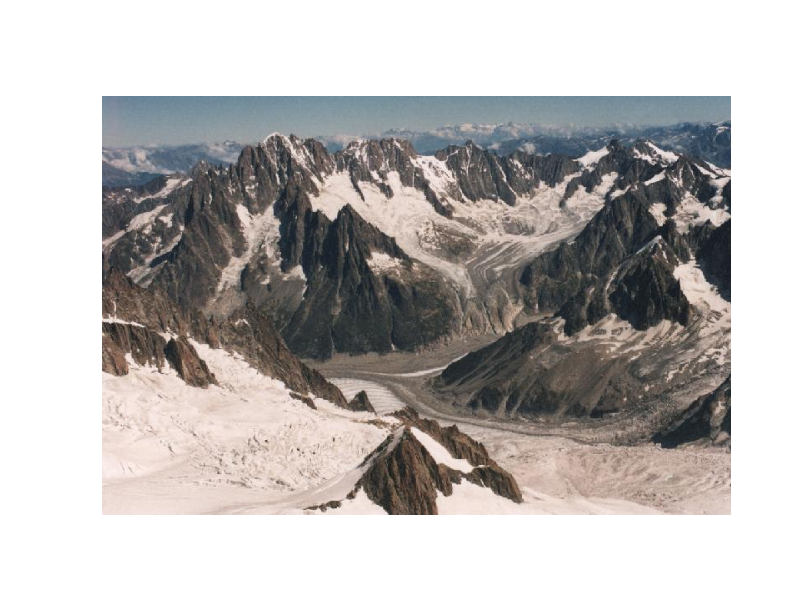
\includegraphics[width=0.45\textwidth]{chpt9_ia/figures/orig.png}
    \label{fig:chpt9:sift_orig}}
  \subfigure[SIFT Keypoints]{
    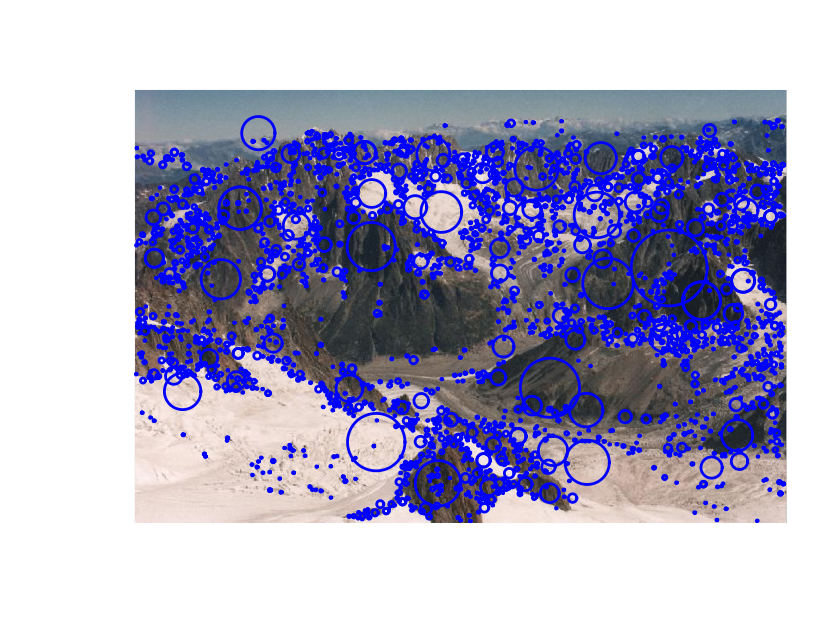
\includegraphics[width=0.45\textwidth]{chpt9_ia/figures/sift.png}
    \label{fig:chpt9:sift_keypoints}}
  \caption{(a) Original image. (b) Original image with SIFT keypoint identification.}
  \label{fig:chpt9:sift}
\end{figure}

When creating a feature vector for a query image, we generate the SIFT features for that
image and then assign each feature to the closest visual word in the training set. Since
we create 1000 clusters, the dimension of our image feature vectors for visual words is
$d_y=1000$. We note that the visual words feature vector is highly dependent on the
training data. Each image's feature vector is dependent on the clusters found in the
training images. Therefore, we cannot pre-compute each image's feature vector without
knowing all training images.

We follow the implementation of visual words provided in \cite{solem2012programming} using
some of the code. The main changes we made were applying tf-idf weight to the visual words
and changing how we represent the vocabulary of the visual words. We also make each visual word
feature vector unit norm. For the SIFT implementation, we
use the publicly available C code at {\small{http://www.vlfeat.org/install-shell.html}}. We
made some minor changes to how the visual word implementation interfaced with the SIFT
feature creation. 

\begin{figure}
  \begin{center}
    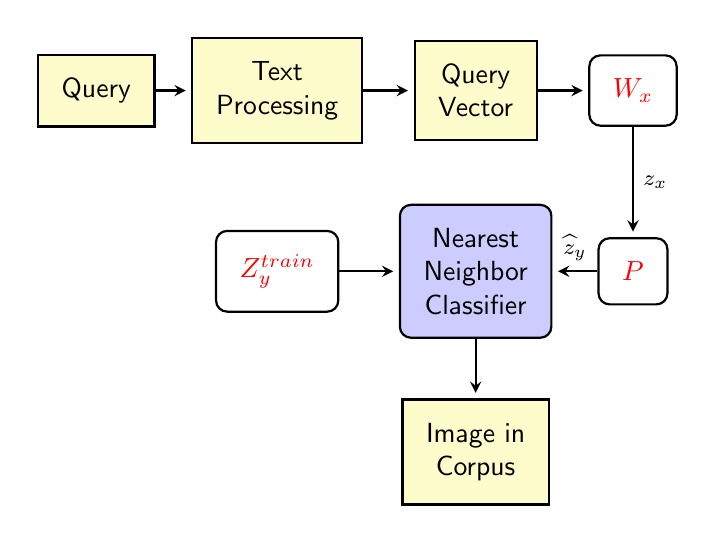
\begin{tikzpicture}[
      font=\sffamily,
      every matrix/.style={ampersand replacement=\&,column sep=3ex,row sep=5ex},
      dataset/.style={draw,thick,fill=yellow!20,inner sep=.3cm},
      sink/.style={dataset,rounded corners,fill=white, text=red},
      app/.style={dataset,rounded corners,fill=blue!20},
      dots/.style={gray,scale=2},
      to/.style={->,>=stealth,shorten >=2pt,thick,font=\sffamily\footnotesize},
      every node/.style={align=center}]

      \matrix{
        \node[dataset] (query) {Query};
        \& \node[dataset] (tp) {Text\\Processing};
        \& \node[dataset] (qv) {Query\\Vector};
        \&;\node[sink] (wx) {$W_x$};  \\

        ; 
        \& \node[sink] (zy) {$Z_y^{\text{train}}$}; 
        \& \node[app] (nn) {Nearest\\Neighbor\\Classifier};
        \& \node[sink] (P) {$P$}; \\

        ; 
        \& ;
        \& \node[dataset] (image) {Image in\\Corpus};
        \& \\
      };

      \draw[to] (query) -- (tp)node[midway,left] {};
      \draw[to] (tp) -- (qv)node[midway,right] {};
      \draw[to] (qv) -- (wx) node[midway,left] {};
      \draw[to] (wx) -- (P) node[midway,right] {$z_x$};
      \draw[to] (P) -- (nn) node[midway,above] {$\widehat{z}_y$};
      \draw[to] (zy) -- (nn) node[midway,right] {};
      \draw[to] (nn) -- (image) node[midway,right] {};


    \end{tikzpicture}
    \caption{Image retrieval pipeline. This system takes a text query as input and the
      correlation model from the training pipeline and will return relevant images.}
  \label{fig:chpt9:test1}
  \end{center}
\end{figure}

\subsection{Correlation Algorithm}

After the datasets have been processed into a caption data matrix $X$ and an image or
document data matrix $Y$, we train the CCA or ICCA as described in Section
\ref{sec:cca}. Regardless of the correlation algorithm, the output at this stage in the
training pipeline are two linear transformations $W_x\in\reals^{d_x\times k_x}$ and
$W_y\in\reals^{d_y \times k_y}$ and a diagonal matrix of canonical correlations,
$P\in\reals^{k_x\times k_y}$. The parameters $k_x$ and $k_y$ are the number of canonical
vectors to use for each dataset, respectively. As any uncorrelated canonical vectors carry
no prediction power, we simply set the number of parameters to $k=k_x=k_y$ and so $P$ is a
square matrix.

Once we learn the canonical basis vectors $W_x$ and $W_y$, we then form
the dimensionality reduced datasets of canonical variates. This is accomplished with the
simple linear transformations
\be
Z_x = W_x^TX\,\,\,\,\,\,\, Z_y = W_y^TY
\ee
where $Z_x\in\reals^{k_x\times n}$ and $Z_y\in\reals^{k_y\times n}$. These are
dimensionality reduced datasets that are maximally correlated. The beauty of these
correlation algorithms is that by solving for $W_x$, $W_y$ and $P$, we automatically solve
a regression problem in the domain of the canonical variates. This relationship is given by
\be
\E{w_x\,|\,w_y} = Pw_y \, \text{ and } \E{w_y\,|\,w_x} = Pw_x.
\ee
Notice that there is no linear offset needed as the datasets are zero mean. We also note
that this above equation is correct and that in both predictions we scale down the known
canonical variate. This makes sense by considering the following example. If $\rho_i=1$, then the
variates $w_x^{i}$ and $w_y^{i}$ are perfectly correlated and predict each other:
$w_x=w_y$. However if $\rho_i=0$, then the variates contain no information and the best
guess that we have is the mean, which is zero. For any $0<\rho_i<1$, we scale the
prediction toward zero depending on the strength of the correlation.

\begin{figure}
  \begin{center}
    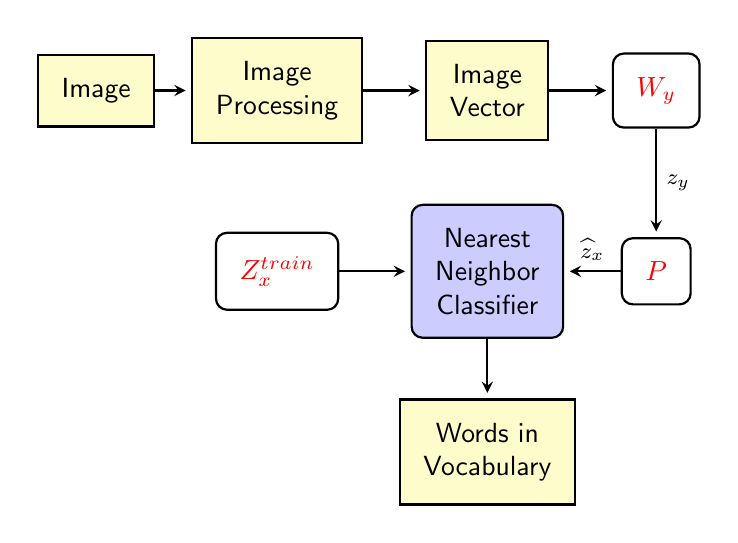
\begin{tikzpicture}[
      font=\sffamily,
      every matrix/.style={ampersand replacement=\&,column sep=3ex,row sep=5ex},
      dataset/.style={draw,thick,fill=yellow!20,inner sep=.3cm},
      sink/.style={dataset,rounded corners,fill=white, text=red},
      app/.style={dataset,rounded corners,fill=blue!20},
      dots/.style={gray,scale=2},
      to/.style={->,>=stealth,shorten >=2pt,thick,font=\sffamily\footnotesize},
      every node/.style={align=center}]


      \matrix{
        \node[dataset] (query) {Image};
        \& \node[dataset] (tp) {Image\\Processing};
        \& \node[dataset] (qv) {Image\\Vector};
        \&;\node[sink] (wx) {$W_y$};  \\

        ; 
        \& \node[sink] (zy) {$Z_x^{\text{train}}$}; 
        \& \node[app] (nn) {Nearest\\Neighbor\\Classifier};
        \& \node[sink] (P) {$P$}; \\

        ; 
        \& ;
        \& \node[dataset] (image) {Words in\\Vocabulary};
        \& \\
      };

      \draw[to] (query) -- (tp)node[midway,left] {};
      \draw[to] (tp) -- (qv)node[midway,right] {};
      \draw[to] (qv) -- (wx) node[midway,left] {};
      \draw[to] (wx) -- (P) node[midway,right] {$z_y$};
      \draw[to] (P) -- (nn) node[midway,above] {$\widehat{z}_x$};
      \draw[to] (zy) -- (nn) node[midway,right] {};
      \draw[to] (nn) -- (image) node[midway,right] {};


    \end{tikzpicture}
    \caption{Image annotation pipeline when using the raw image as input. This system
      takes an image and correlation model from the training system as inputs and will
      return a list of words that are most relevant for the image.}
  \label{fig:chpt9:test2}
  \end{center}
\end{figure}

\begin{figure}
  \begin{center}
    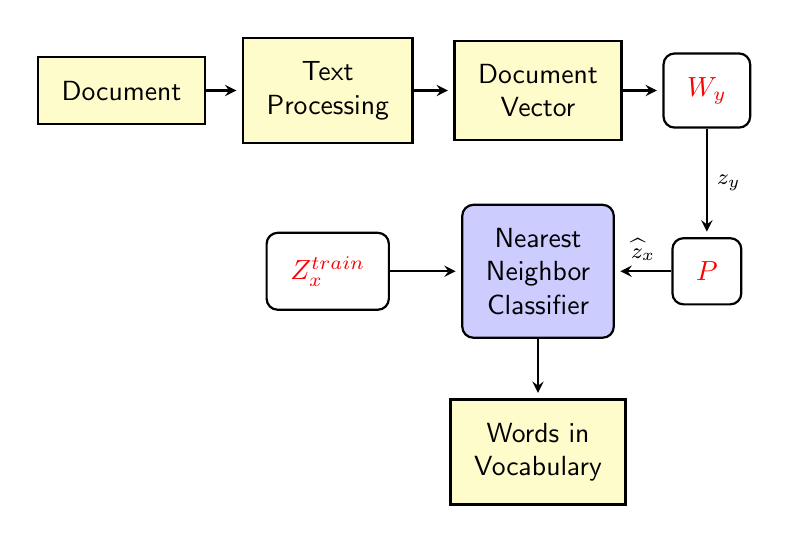
\begin{tikzpicture}[
      font=\sffamily,
      every matrix/.style={ampersand replacement=\&,column sep=3ex,row sep=5ex},
      dataset/.style={draw,thick,fill=yellow!20,inner sep=.3cm},
      sink/.style={dataset,rounded corners,fill=white, text=red},
      app/.style={dataset,rounded corners,fill=blue!20},
      dots/.style={gray,scale=2},
      to/.style={->,>=stealth,shorten >=2pt,thick,font=\sffamily\footnotesize},
      every node/.style={align=center}]


      \matrix{
        \node[dataset] (query) {Document};
        \& \node[dataset] (tp) {Text\\Processing};
        \& \node[dataset] (qv) {Document\\Vector};
        \&;\node[sink] (wx) {$W_y$};  \\

        ; 
        \& \node[sink] (zy) {$Z_x^{\text{train}}$}; 
        \& \node[app] (nn) {Nearest\\Neighbor\\Classifier};
        \& \node[sink] (P) {$P$}; \\

        ; 
        \& ;
        \& \node[dataset] (image) {Words in\\Vocabulary};
        \& \\
      };

      \draw[to] (query) -- (tp)node[midway,left] {};
      \draw[to] (tp) -- (qv)node[midway,right] {};
      \draw[to] (qv) -- (wx) node[midway,left] {};
      \draw[to] (wx) -- (P) node[midway,right] {$z_y$};
      \draw[to] (P) -- (nn) node[midway,above] {$\widehat{z}_x$};
      \draw[to] (zy) -- (nn) node[midway,right] {};
      \draw[to] (nn) -- (image) node[midway,right] {};


    \end{tikzpicture}
    \caption{Image annotation pipeline when using associated text documents. This system
      takes a text document and correlation model from the training system as inputs and will
      return a list of words that are most relevant for the associated image.}
  \label{fig:chpt9:test3}
  \end{center}
\end{figure}


\subsection{Image Retrieval}

After training the system on a corpus, a user may perform image retrieval. Given a text
query, we first process it using the same tf-idf weighting scheme used in the training
model, resulting in the vector $q\in\reals^{d_x\times 1}$. To obtain an estimate of our
image feature, we perform the following sequence of linear transformations, learned by one
of the correlation algorithms,
\be
\widehat{z}_y = PW_x^Tq
\ee
To return relevant images, we use a nearest neighbor classifier in the canonical variate
domain. We can pre-compute all possible images to return via $Z_y^{\text{train}} = W_y^TY$.
The output of the search is 
\beq\label{eq:chpt9:ir_scores} y_{\text{guess}} =
\argmin_{z_y\in Z_y^{\text{train}}}
\|z_y-\widehat{z}_y\|_2^2,
\eeq
which is repeated for as many results the user desires, excluding previously returned
results from the search set each time. A nice benefit of using correlation methods is that
additional images may be added to the set of returnable images, even if they do not have a
caption associated with them. All we need is the low dimensional representation of these
additional images using the transformation learned from the training set, whether that be
image features or document vectors.

\subsection{Image Annotation}

The trained system can also handle automatic image annotation. Given a query image or
associated document, we
first process it using the same image or text processing that was used in training, resulting in a
query vector $q\in\reals^{d_y\times 1}$. To obtain an estimate of our text features, we
perform the following linear transformation
\be
\widehat{z}_x = PW_y^Tq
\ee
using the correlation model learned in the training phase. To return relevant words, we
use a nearest neighbor classifier in the canonical variate domain. However, instead of
using the captions as the vectors to compare against, we consider $d_x$ documents, each of
which contains exactly one of the words in the vocabulary. Let $D\in\reals^{d_x\times
  d_x}$ be a diagonal matrix with entries equal to the tf-idf score of that word. Define
$Z_x^{\text{train}}=W_x^TD$ to be the canonical variate vectors of each word. Then the output of the
nearest neighbor classifier is
\beq\label{eq:chpt9:ia_scores} x_{\text{guess}} =
\argmin_{z_x\in Z_x^{\text{train}}}
\|z_D-\widehat{z}_x\|_2^2.
\eeq 
We then return the words corresponding to the vectors returned by the nearest neighbor
classifier.

\section{Experiments}\label{sec:results}

To compare the performance of CCA and ICCA in image retrieval and annotation, we test our
system on four different datasets. For the Pascal Image Dataset, we wrote a command line
interface to perform both image retrieval and image annotation. This allows for us to
qualitatively determine how each method works. For the University of Washington Ground
Truth dataset, we run the training and testing pipelines in Figures
\ref{fig:chpt9:training} and \ref{fig:chpt9:test2} and compare the R-precision for the
image annotation task. For the Gold Standard Web dataset, we only have a few image-caption
pairs but also have associated text documents and so we use the training pipelines in
Figures \ref{fig:chpt9:training_tt} and \ref{fig:chpt9:test3}. We compare our eigen-based
annotation methods to previous NLP methods using the evaluation framework in
\cite{leong2010text}. Finally, we use the training pipelines in Figures
\ref{fig:chpt9:training_tt} and \ref{fig:chpt9:test3} to test the image annotation
performance of CCA and ICCA on the BBC News dataset. This dataset is particularly
challenging first because the images are extremely varied and may only be tangentially
related to the associated document, and second because the accompanying caption is often
extremely nuanced, containing few keywords. These challenges present many latent
variables, which CCA and ICCA will not handle very well.

\subsection{Pascal Image Dataset}

\begin{figure}[t]
  \begin{minipage}{0.45\linewidth}
    \centering
    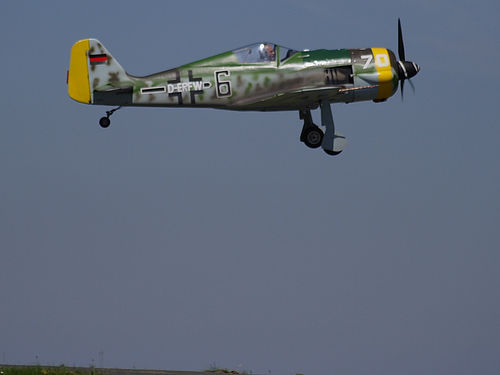
\includegraphics[width=.8\textwidth]{chpt9_ia/figures/img_3.jpg}
  \end{minipage}
  \begin{minipage}[t]{0.45\linewidth}
    \vspace{-1in}
    \centering
    \footnotesize
    \begin{itemize}
    \item A D-ERFW-6 in flight.
    \item An army green plane flying in the sky.
    \item An old fighter plane flying with German military markings.
    \item A small green and yellow plane in the sky.
    \item A WWII fighter plane with its landing gear down.
    \end{itemize}
  \end{minipage}
  \caption{Example of an image and its captions in the Pascal dataset}
  \label{fig:chpt9:pascal}
\end{figure}

The Pascal Image dataset
\footnote{http://nlp.cs.illinois.edu/HockenmaierGroup/pascal-sentences/} was created using
Amazon's Mechanical Turk \cite{rashtchian2010collecting}. The dataset consists of 1000
images, each with 5 captions. The average image has 26.67 caption words and the total
vocabulary size of the corpus is 2393. The 5 captions for each image are unique, but they
may repeat keywords or use synonyms.  For example, airplanes in the dataset can be
described as airplanes, planes, fighter planes, jets, and even their model. See Figure
\ref{fig:chpt9:pascal} for an example image-caption pair.

\begin{figure}[t]
  \centering
  \subfigure[CCA Results]{
    \centering
    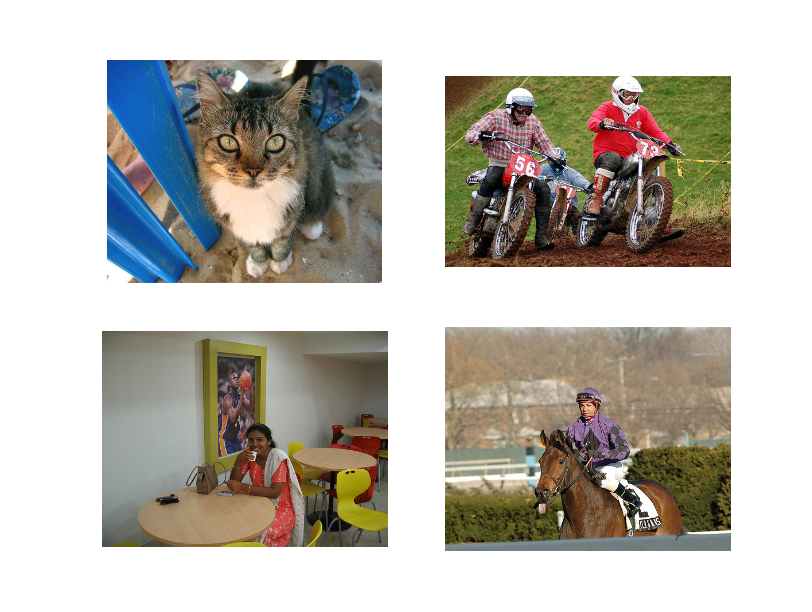
\includegraphics[width=0.45\textwidth]{chpt9_ia/figures/pascal_cca_ex.png}
    \label{fig:chpt9:CCA_query_results}}
  \subfigure[ICCA Results]{
    \centering
    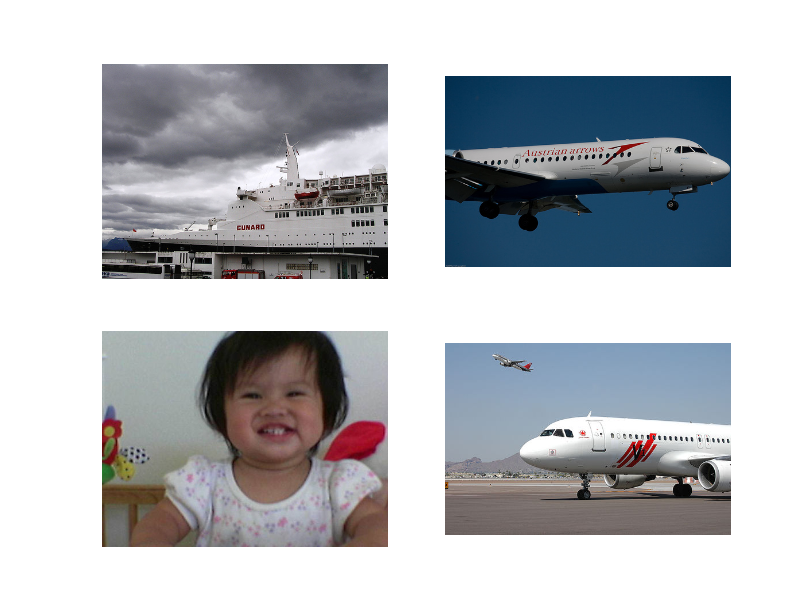
\includegraphics[width=0.45\textwidth]{chpt9_ia/figures/pascal_icca_ex.png}
    \label{fig:chpt9:ICCA_query_results}}
  \caption{(a) CCA results for query "airplane". (b) ICCA results for query "airplane".}
  \label{fig:chpt9:pascal_results}
\end{figure}

\begin{figure}[t]
  \centering
  \subfigure[CCA Results]{
    \centering
    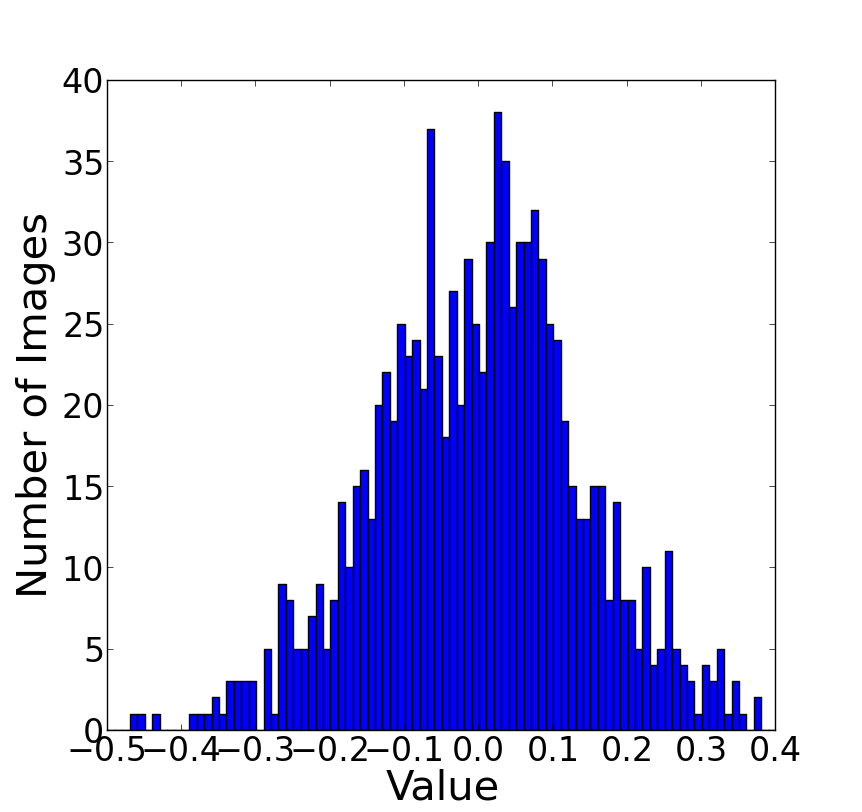
\includegraphics[width=0.45\textwidth]{chpt9_ia/figures/cca_ir.png}
    \label{fig:chpt9:cca_ir}}
  \subfigure[CCA Results Zoomed]{
    \centering
    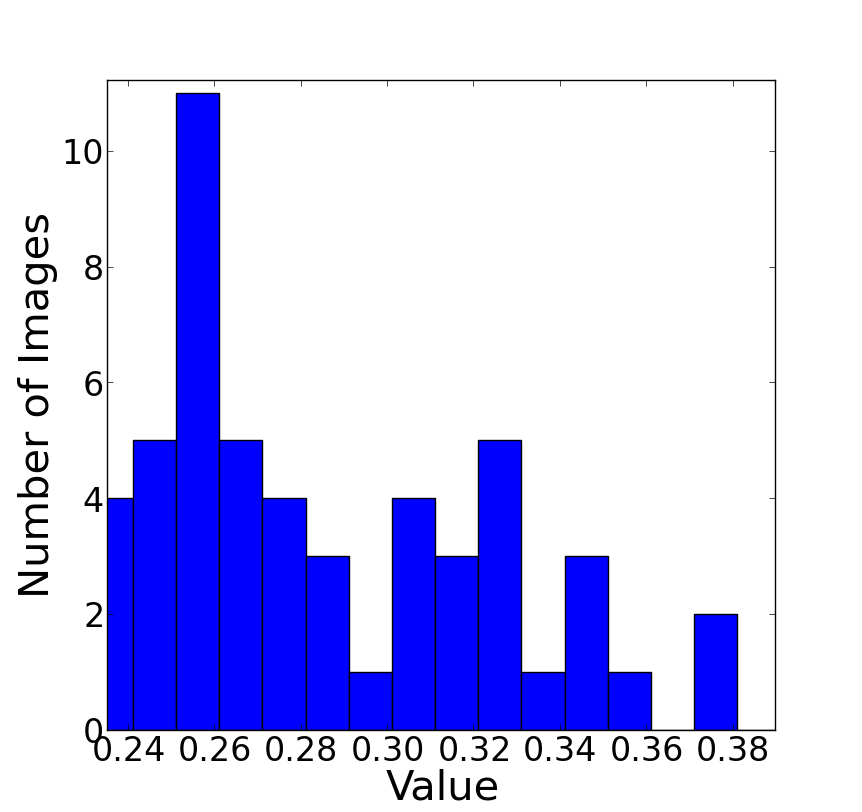
\includegraphics[width=0.45\textwidth]{chpt9_ia/figures/cca_ir_zoom.png}
    \label{fig:chpt9:cca_ir_zoom}}
  \subfigure[ICCA Results]{
    \centering
    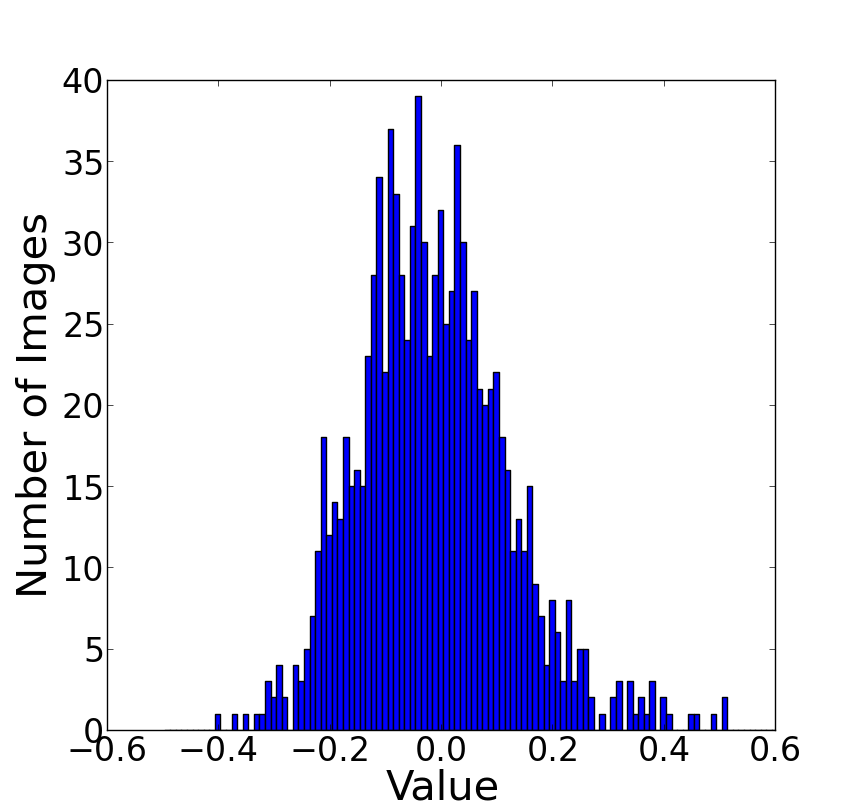
\includegraphics[width=0.45\textwidth]{chpt9_ia/figures/icca_ir.png}
    \label{fig:chpt9:icca_ir}}
  \subfigure[ICCA Results Zoomed]{
    \centering
    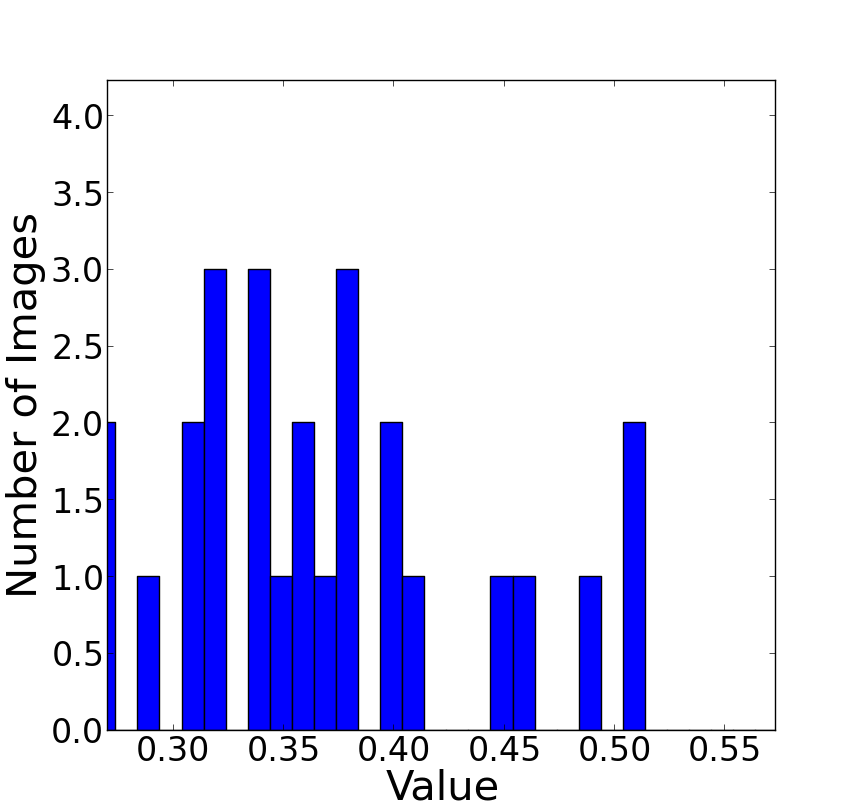
\includegraphics[width=0.45\textwidth]{chpt9_ia/figures/icca_ir_zoom.png}
    \label{fig:chpt9:icca_ir_zoom}}
  \caption{(a) Scores for all 1000 Pascal images for the query ``airplane'' for CCA. (b)
    Zoomed in version of (a) to highlight the top scores returned in Figure
    \ref{fig:chpt9:CCA_query_results}. (c) Scores for all 1000 Pascal
    images for the query ``airplane'' for ICCA. (d) Zoomed in version of (c) to highlight
    the top scores which are returned in Figure \ref{fig:chpt9:ICCA_query_results}. All
    scores are the norm in (\ref{eq:chpt9:ir_scores}).}
  \label{fig:chpt9:pascal_ir}
\end{figure}

To qualitatively evaluate the performance of CCA and ICCA using visual words, we
implemented the image retrieval and image annotation systems described in Section
\ref{sec:propose}. Figure \ref{fig:chpt9:pascal_results} shows the first four images
retrieved for the search query ``airplane'' using both CCA and ICCA correlation models. We
plot the scores used to return these images in Figure \ref{fig:chpt9:pascal_ir}. The
largest four scores correspond to the images in Figure \ref{fig:chpt9:pascal_results} as
computed via (\ref{eq:chpt9:ir_scores}). Figure \ref{fig:chpt9:pascal_annotation} shows
the first ten words returned for the image in Figure \ref{fig:chpt9:pascal_query_image},
which was taken from the Pascal dataset. Figure \ref{fig:chpt9:pascal_ia} plots the
corresponding scores for all words in the database as computed via
(\ref{eq:chpt9:ia_scores}). The top scores correspond to the words returned in Figure
\ref{fig:chpt9:pascal_annotation}. For both tasks, we used all 1000 image-caption pairs in
the Pascal dataset for training. Thus, any image in the dataset may be returned in the
image retrieval task. Similarly, any Porter-stemmed vocabulary word in the entire caption
dataset may be returned in the image annotation task.

\begin{figure}[t]
	\centering
	\subfigure[Image Query] {
	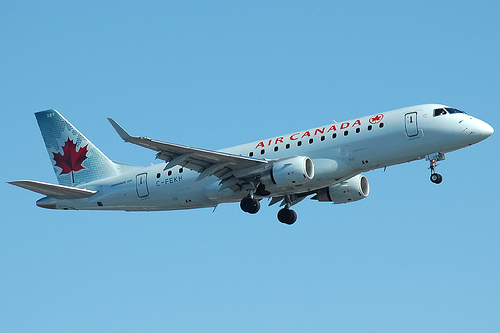
\includegraphics[width=0.4\textwidth]{chpt9_ia/figures/img_27.jpg}
	\label{fig:chpt9:pascal_query_image}}

	\subfigure{
    \begin{minipage}[t]{0.3\textwidth}
      \small
      \begin{center}
        \textbf{CCA Annotation}
      \end{center}
      \begin{enumerate}
      \item hairless
      \item buddi
      \item swan
      \item leaf-less
      \item bnsf
      \item desert
      \item fluffi
      \item salad
      \item majest
      \item memorabilia
      \end{enumerate}
    \end{minipage}%
    \begin{minipage}[t]{0.2\textwidth}
    \end{minipage}
    \begin{minipage}[t]{0.3\textwidth}
      \small
      \begin{center}
        \textbf{ICCA Annotation}
      \end{center}
      \begin{enumerate}
      \item plane
      \item ship
      \item cruis
      \item fly
      \item blue
      \item jet
      \item airplan
      \item dock
      \item fighter
      \item through
      \end{enumerate}
    \end{minipage}}
	\caption{CCA vs ICCA annotation results for the image query shown in
      \ref{fig:chpt9:pascal_query_image}.}
    \label{fig:chpt9:pascal_annotation}
\end{figure}

\begin{figure}[t]
  \centering
  \subfigure[CCA Results]{
    \centering
    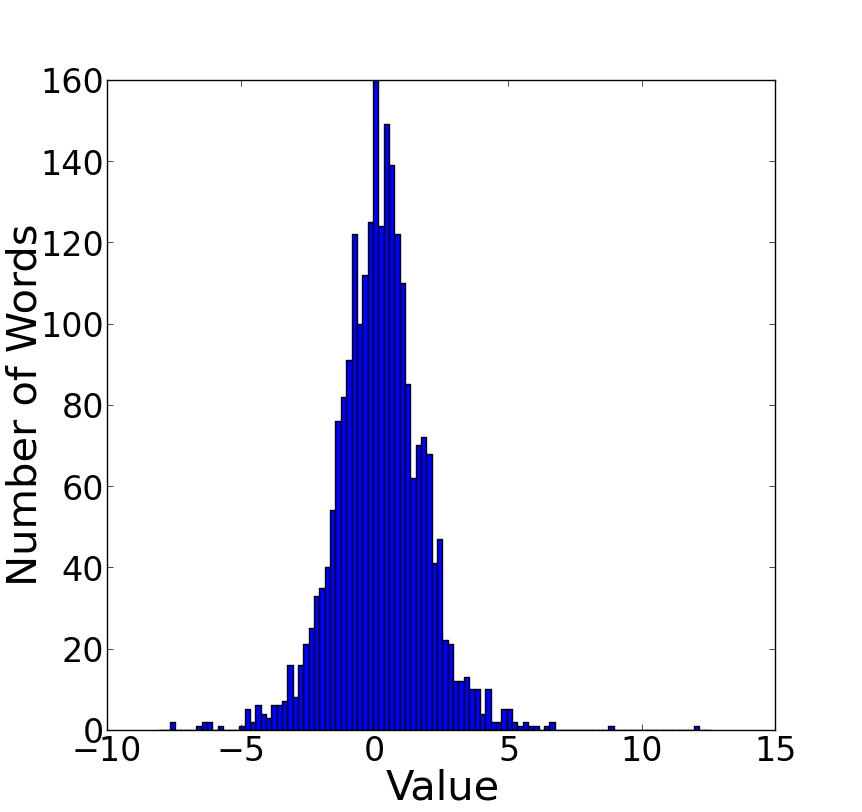
\includegraphics[width=0.45\textwidth]{chpt9_ia/figures/cca_ia.png}
    \label{fig:chpt9:cca_ia}}
  \subfigure[CCA Results Zoomed]{
    \centering
    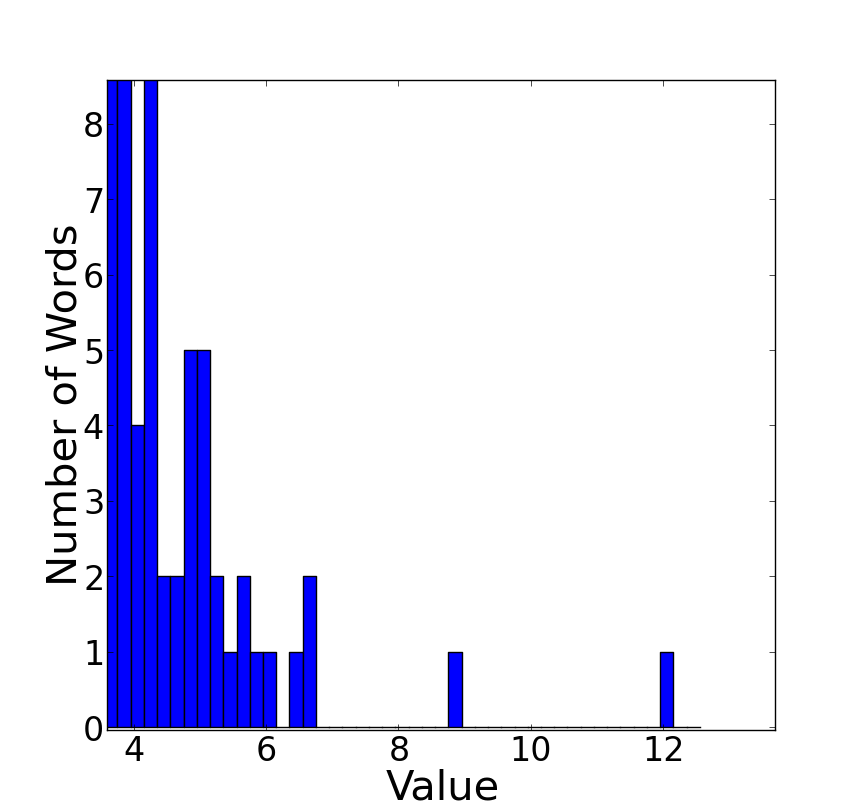
\includegraphics[width=0.45\textwidth]{chpt9_ia/figures/cca_ia_zoom.png}
    \label{fig:chpt9:cca_ia_zoom}}
  \subfigure[ICCA Results]{
    \centering
    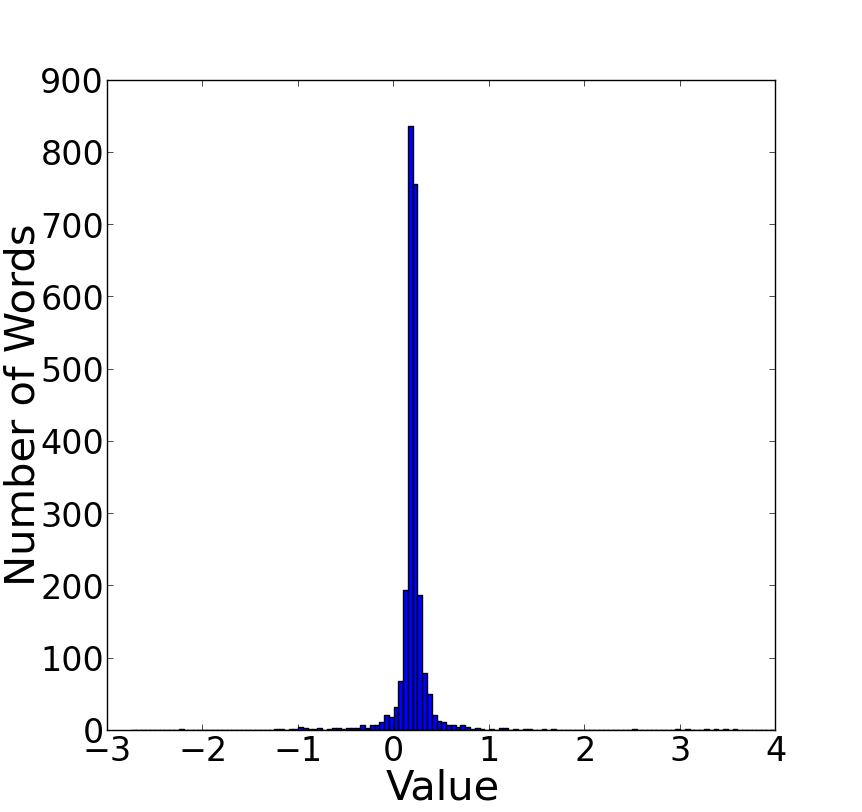
\includegraphics[width=0.45\textwidth]{chpt9_ia/figures/icca_ia.png}
    \label{fig:chpt9:icca_ia}}
  \subfigure[ICCA Results Zoomed]{
    \centering
    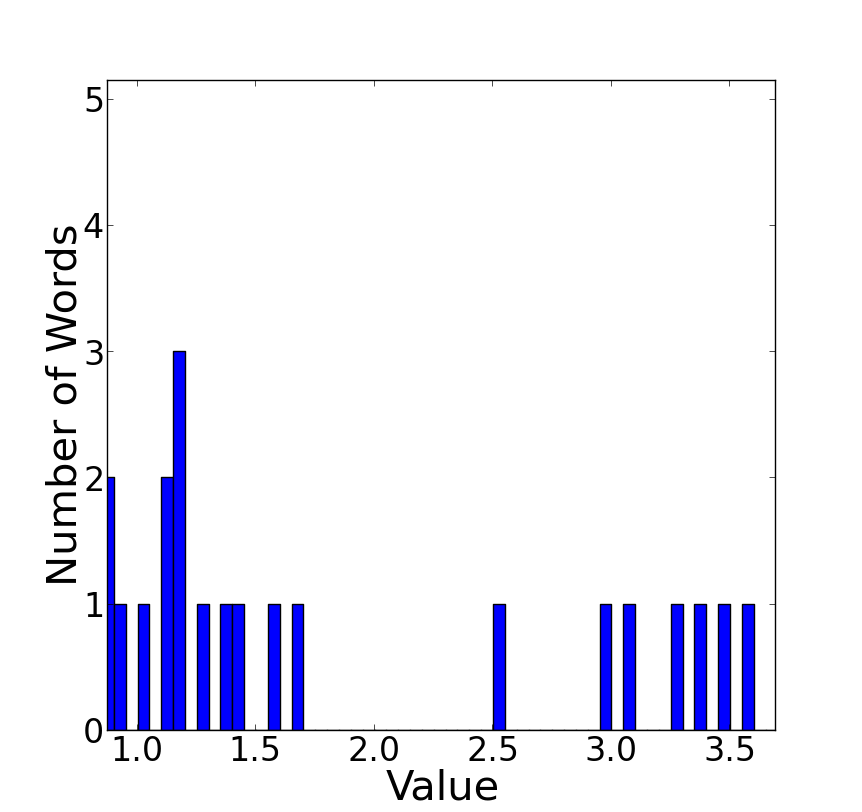
\includegraphics[width=0.45\textwidth]{chpt9_ia/figures/icca_ia_zoom.png}
    \label{fig:chpt9:icca_ia_zoom}}
  \caption{(a) CCA scores for all words in the Pascal database for the image query in
    Figure \ref{fig:chpt9:pascal_query_image}. (b) Zoomed in version of (a) to highlight
    the top scores returned in Figure \ref{fig:chpt9:pascal_annotation}. (c) ICCA scores
    for all words in the Pascal database for the image query in Figure
    \ref{fig:chpt9:pascal_query_image}. (d) Zoomed in version of (c) to highlight the top
    scores which are returned in Figure \ref{fig:chpt9:pascal_annotation}. All
    scores are the norm in (\ref{eq:chpt9:ia_scores}).}
  \label{fig:chpt9:pascal_ia}
\end{figure}

\subsection{Ground Truth Image Dataset}

To quantitatively compare the performance of CCA and ICCA, we used the University of
Washington Ground Truth Image Dataset
\footnote{http://www.cs.washington.edu/research/imagedatabase/groundtruth/}. This
dataset contains 1109 images with an average of 5.57 keywords per image and a total of 346
unique words. We randomly split the dataset into 3 sets: a training set of 550 images, a
validation set of 250 images and a testing set of 309 images. This was repeated to obtain
10 such partitions.

For each partitioning, the training dataset was used to learn the correlation model for
CCA, and ICCA. This model was learned for values of $k=$10,25,50,75,100.  The validation
dataset was then used to determine the best value of $k$ for each algorithm, using
R-precision as our evaluation metric. In this setting, R-precision is equal to the
percentage of correctly predicted keywords for an image. Once the best $k$ was determined,
that partition's R-precision value for each algorithm was determined on the testing
datasets. The R-precision values were then averaged across partitions. Figure
\ref{fig:chpt9:gt_rprec} plots the probability density function of R-precision for CCA and
ICCA and Table \ref{table:rprec} shows the mean R-precision and average $k$
values.

\begin{figure}[t]
  \centering
  \subfigure[CCA]{
    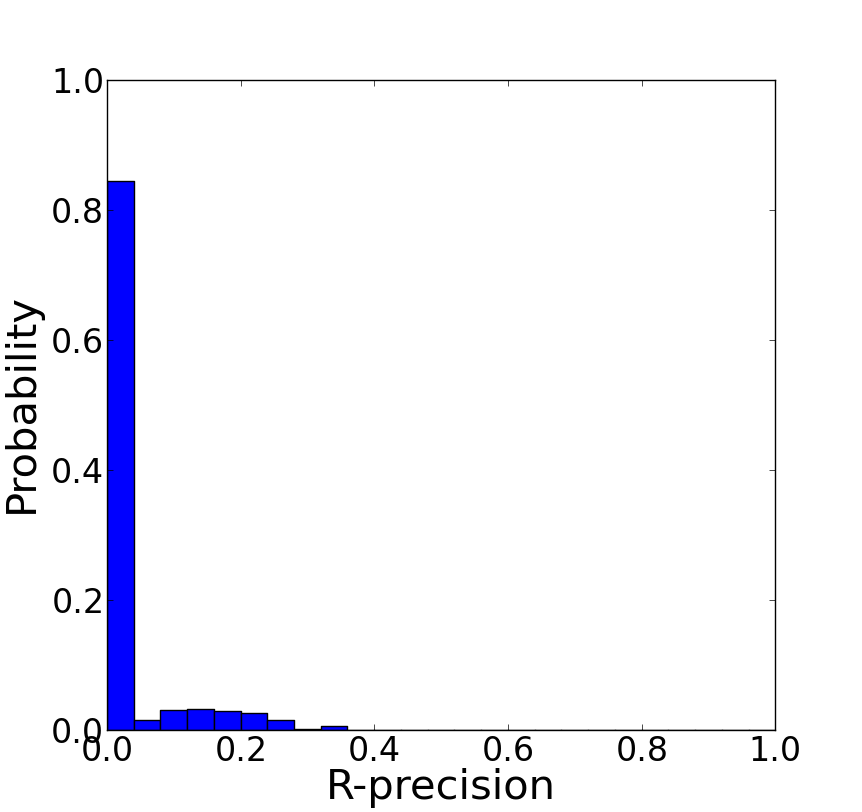
\includegraphics[width=0.45\textwidth]{chpt9_ia/figures/cca_rprec_vw.png}
    \label{fig:chpt9:rprec_cca_vw}}
  \subfigure[ICCA]{
    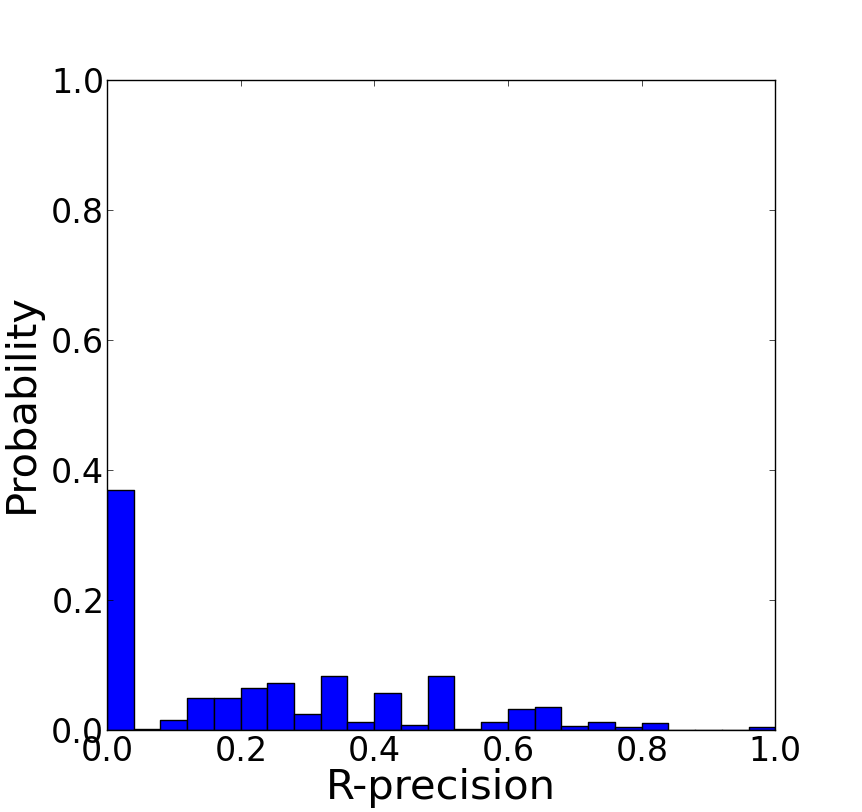
\includegraphics[width=0.45\textwidth]{chpt9_ia/figures/icca_rprec_vw.png}
    \label{fig:chpt9:rprec_icca_vw}}
  \caption{Empirical probability density functions of R-precision of image annotation of
    the University of Washington Ground Truth Dataset.}
  \label{fig:chpt9:gt_rprec}
\end{figure}

\begin{table}[t]
\centering
\begin{tabular}{c||c|c}
& Mean R-precision& Mean $k$\\ \hline
CCA &  0.024& 63\\
ICCA & 0.232& 20\\
\bottomrule
\end{tabular}
\caption{Average R-precision values and correlation basis dimension, $k$, for image
  annotation of the University of Washington  Ground Truth Dataset }
\label{table:rprec}
\vspace{-0.1in}
\end{table}

\subsection{Gold Standard Web Dataset}

Next, we evaluate our eigen-based image annotation methods on the Gold Standard Web
Dataset \cite{leong2010text}. This dataset contains 300 image-text pairs that was
collected from the web. The average text document length is 278 tokens and the vocabulary
size is 8,409 words. Each image also has a gold standard of manually assigned tags labeled
by five human annotators. We consider these manually assigned tags as the
caption. However, as we only have 300 images and these images contain many different
objects, we use the associated text document  as the second
modality. Hence, our goal is to predict the captions given the text document, which is
essentially keyword identification.

We use the same four evaluation metrics as \cite{leong2010text} to be able to make direct
comparisons with previous methods. As CCA and ICCA can return an arbitrary number of
keywords, we choose to always predict keywords equal to the number of true
keywords. Therefore, for our methods, these metrics are variations on R-precision. Some
images are considered Mode images when there is a unique keyword selected by more
annotators than any other keyword. The metrics are given in Table
\ref{table:gold_metrics}. Let $\mathcal{I}$ be the set of all images, $\mathcal{IM}$ be
the set of mode images, $f_i^j$ be the number annotators who labeled image $i$ with keyword
$j$, $r_i$ be the number of keywords selected for image $i$, and $R_i=\sum_{j=1}^{r_i}f_i^j$. Table \ref{table:gold}
reports the performance of CCA and ICCA in generating keywords given these 4 metrics using
leave-one-out testing. We also provide the performance of models used in
\cite{leong2010text} for comparison.

\begin{table}[t]
  \centering
  \begin{tabular}{l|l}
    Metric & Expression\\
    \midrule
    Best Normal & $\frac{1}{|\mathcal{I}|}\sum_{i\in\mathcal{I}}\frac{1}{r_iR_i}\sum_{j=1}^{r_i}f_i^j$\\
    Best Mode & $\frac{1}{|\mathcal{IM}|}\sum_{i\in\mathcal{IM}}\indicator_{\left\{\text{top tag = mode}\right\}}$\\
    oot Normal & $\frac{1}{|\mathcal{I}|}\sum_{i\in\mathcal{I}}\frac{1}{R_i}\sum_{j=1}^{r_i}f_i^j$\\
    oot Mode & $\frac{1}{|\mathcal{IM}|}\sum_{i\in\mathcal{IM}}\indicator_{\left\{\text{any tag = mode}\right\}}$\\
    \bottomrule
  \end{tabular}
  \caption{Image annotation for the Web Image-Article dataset.}
  \label{table:gold_metrics}
  \vspace{-0.1in}
\end{table}


\begin{table}[t]
\centering
\begin{tabular}{l|cc|cc}
Models & Best Normal & Best Mode & oot Normal & oot Mode\\\hline
CCA & 0.01 & 0.00 & 1.49 & 35.23\\
ICCA & 0.19 & 9.09 & 16.11 & 76.7 \\
\midrule
\midrule
Flickr picturability & 6.32 & 78.57 & 35.61 & 92.86\\
Wikipedia Salience & 6.40 & 7.14 & 35.19 & 92.86 \\
Topic modeling & 5.99 & 42.86 & 37.13 & 85.71 \\
\midrule
\midrule
Doc Title & 6.40 & 75.00 & 18.97 & 82.14\\
tf*idf & 5.94 & 14.29 & 38.40 & 78.57\\
\bottomrule
\end{tabular}
\caption{Image annotation for the Web Image-Article dataset.}
\label{table:gold}
\vspace{-0.1in}
\end{table}


\subsection{BBC News Dataset}

Finally, we evaluate CCA and ICCA based image annotation on the BBC News dataset
\cite{feng2008automatic}. Similar to the Gold Standard Web dataset, this dataset contains
image-caption-document tuples that are separated into 3121 training examples and 240
testing examples. The images in this dataset are again very varied and the captions are
sometimes nuanced and very specific to the image and not very related to the accompanying
document. For the CCA and ICCA annotations, we again will use the accompanying documents
to predict keywords in the caption. We report the precision and recall when returning the
top 10, 15 and 20 predicted keywords in Table \ref{table:bbc}. In the table we also report
methods from \cite{feng2008automatic} and \cite{leong2010text} for comparison.  We follow
implementations reported in \cite{feng2008automatic} and \cite{leong2010text} to not
Porter stem the words but instead use Tree Tagger\cite{schmid1994probabilistic} to include
only nouns, verbs, and adjectives.

\begin{figure}[t]
  \begin{minipage}{0.45\linewidth}
    \centering
    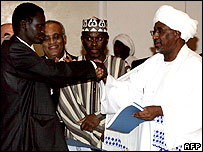
\includegraphics[width=.8\textwidth]{chpt9_ia/figures/bbc_img.jpg}
  \end{minipage}
  \begin{minipage}{0.45\linewidth}
    \centering
    \footnotesize
    \textbf{Caption}
    \begin{itemize}
    \item Agreement came despite reservations on both sides
    \end{itemize}
    \textbf{Title}
    \begin{itemize}
    \item UN Secretary General Kofi Annan has called on the Sudanese government to allow a
      UN assessment team into the war-torn region of Darfur
    \end{itemize}
  \end{minipage}
  \caption{Example of an image, its caption, and title in the BBC News dataset}
  \label{fig:chpt9:bbc_ex}
\end{figure}


\begin{table}[t]
\centering
\begin{tabular}{l|cc|cc|cc}
& \multicolumn{2}{|c|}{Top 10} & \multicolumn{2}{|c|}{Top 15} & \multicolumn{2}{|c|}{Top
  20}\\
Models & P & R & P & R & P & R\\ 
\midrule
CCA & 0.08 & 0.11 & 0.08 & 0.22 & 0.08 & 0.28\\
ICCA & 0.79 & 1.48 & 0.72 & 1.95 & 0.73 & 2.63\\
\midrule
\midrule
tf*idf & 4.37 & 7.09 & 3.57 & 8.12 & 2.65 & 8.89\\
DocTitle & 9.22 & 7.03 & 9.22 & 7.03 & 9.22 & 7.03\\
Lavrenko03 & 9.05 & 16.01 & 7.73 & 17.87 & 6.55 & 19.38\\
ExtModel & 14.72 & 27.95 & 11.62 & 32.99 & 9.72 & 36.77\\
\midrule
\midrule
Flickr picturability & 12.13 & 22.82 & 9.52 & 26.82 & 8.23 & 29.80\\
Wikipedia Salience & 11.63 & 21.89 & 9.28 & 26.20 & 7.81 & 29.41\\
Topic Modeling & 11.42 & 21.49 & 9.28 & 26.20 & 7.86 & 29.57\\
\bottomrule
\end{tabular}
\caption{Image annotation for the Web Image-Article dataset.}
\label{table:bbc}
\vspace{-0.1in}
\end{table}

\section{Discussion}\label{sec:disc}
\subsection{Pascal Results}

For the Pascal dataset, we can qualitatively see the performance increase that ICCA
gives. Examining Figure \ref{fig:chpt9:CCA_query_results}, we see that CCA returns random
images associated with the query ``airplane''. This is the case with any other query
entered.  However this is expected with CCA as it returns a correlation of 1 between all
images and tokens as we are operating in the sample deficient regime.  Any positive
results returned by CCA can be attributed to random luck. On the other hand, using ICCA to
train a retrieval system results in better overall performance than CCA. This can be seen
specifically in Figure \ref{fig:chpt9:ICCA_query_results}, which shows images for the same
query of ``airplane''. Using ICCA, two of the first four results are planes. By only using
\textit{informative} singular vectors, ICCA is able to return more relevant images.

Specifically, if we examine Figure \ref{fig:chpt9:pascal_ir}, we can compare the scores
returned for each image for CCA and ICCA. The top scores for ICCA seem to separate from
the bulk of the others, while for CCA, the top scores seem to be part of the bulk
distribution. This gives support to the notion that ICCA is able to identify images that
are relevant to the desired keyword.

Image annotation using CCA also returns random keywords for any image query. An example of
this is shown in Figure \ref{fig:chpt9:pascal_annotation}. The query image is an airplane but
the top 10 words returned by CCA are all irrelevant. This once again reinforces the idea
that CCA only returns random results in the sample deficient regime. However, examining
the top 10 words returned by ICCA for the same image, we observe meaningful annotations
such as ``plane'', ``blue'', ``fly''. Examining Figure \ref{fig:chpt9:pascal_ia}, we see the
corresponding scores to the words returned in Figure
\ref{fig:chpt9:pascal_annotation}. Again we notice that a majority of the words fall into
the bulk distribution for CCA and ICCA. The words in the bulk part of the distribution are
not informative. However, in ICCA, there are a number of words that separate from the bulk
distribution, which we show in Figure \ref{fig:chpt9:pascal_annotation}. However, the
scores for CCA do not separate as nicely from the distribution. This further gives support
that CCA randomly returned words/images in the sample deficient regime.

A \naive image retrieval system may perform a search using only the captions and then
return the image associated with the most notable caption. This produces very good results
for the Pascal dataset because the captions are very clean and noise-free. Every caption
with the word sheep will have a sheep in the image. However, correlation based approaches
have a few main advantages over such a \naive method. First, correlation methods solve
both the image retrieval and image annotation problem simultaneously. The \naive image
retrieval method cannot solve the image annotation problem. Second, correlation methods
can handle adding images to the corpus post training, even if it does not have an
associated caption. For the image retrieval problem, the correlation methods will return
images with low-dimensional representation that are close to the predicted vector. Adding
additional images (even without captions) requires transforming the images into the
low-dimensional representation using the trained transformation and then adding them to
the set of possible images to be returned. The \naive method needs a caption for every
image and if a new image-caption pair was added, the entire inverted index and vocabulary
would need to be recomputed.


\subsection{Image Annotation of Ground Truth Dataset}

We use the Ground Truth Dataset to provide a more quantitative comparison of CCA and ICCA
based image annotation. The captions for this dataset only consist of keywords and is
thus easier to assess the quality of the image annotations. We did not clean up the
dataset by removing misspelled words or words appearing only once. Therefore, the reported
results are a nice lower-bound that one could expect by doing such clever pre-processing
steps. As evident in Table \ref{table:rprec}, CCA performs very poorly on the image
annotation task. This R-precision corresponds to random guessing, which matches the
results of \cite{pezeshki2004empirical} stating that in the sample starved regime, the CCA
bases are random projections. However, using ICCA to informatively trim data matrices
results in improved annotations. Examining the figures in Figure \ref{fig:chpt9:gt_rprec}, we
see that when using CCA, approximately 85\% of the images result is an R-precision of
0. However, ICCA returns zero relevant images only 35\% of the time. Clearly, ICCA is able
to uncover true correlations to return relevant annotations. This gives credence to using
correlation methods for image annotation tasks.

\subsection{Annotation of Gold Standard Web Dataset}

The Gold Standard Web dataset is a more difficult dataset than the Ground Truth
dataset. First, there are only 300 examples in the dataset. Using leave-one-out testing
gives a training dataset of only 299 examples. Second, the dimensions of our dataset
increases because we use tf-idf weights from the associated documents instead of visual
words from the image. Therefore, we are in a very sample deficient regime where our
dimension of each dataset is on the order of 8000 and we only have 299
samples. Compounding issues, these vectors are very sparse as documents only have a subset
of the total words in the vocabulary. However, ICCA is indeed able to recover meaningful
annotations even in this regime.

Examining the difference between the Best Mode and oot Mode performance metrics, we see
that ICCA has a very large gap. This indicates that the ICCA retrieval method is very
often able to retrieve the mode annotation, just not label it as the best annotation. 

\subsection{Annotation of BBC News Dataset}

The BBC News dataset is the most difficult dataset we consider in this chapter. Here, we
have a large number of training data, however, our captions are very ``noisy''. Unlike the
Gold Standard Web dataset, the BBC captions may contain words that do not appear in the
accompanying document. These captions are also very nuanced and may describe an image that
is only tangentially related to the main article. For example, consider Figure
\ref{fig:chpt9:bbc_ex}. The image is of two men shaking hands, however, the caption
describes this very abstractly. In addition, the caption highlights a very subtle point of
the main article, as we can see by the title. Similar to the Gold Standard Web dataset,
our feature vectors are both very high dimensional and sparse. We see from the results in
Table \ref{table:bbc} that both CCA and ICCA do a poor job at retrieving relevant
annotations given the BBC article. However, we do observe the behavior that CCA returns
completely random results and ICCA is able to perform slightly better (non-randomly).

The BBC News dataset breaks many of the assumptions of ICCA and therefore causes its
performance to decrease. First, the dataset breaks the linear correlation assumption of
ICCA. As we saw in Figure \ref{fig:chpt9:bbc_ex}, captions are can be very nuanced, indicating
many latent variables interacting in most likely nonlinear ways. Due to the size of the
vocabulary of the BBC dataset, our text feature vectors are incredibly sparse, which as we
saw in previous chapters, requires a larger SNR to detect correlations. The nonlinear
correlations most certainly decrease the SNR in our dataset, which, coupled with the
sparse data, stretches ICCA based image annotation to the limit of decent operation. 

Clever feature engineering and alterations of ICCA could yield potential new avenues to
improve the performance on difficult datasets such as the BBC News dataset. One possible
extension is to use a kernel version of ICCA to account for nonlinear
correlations. Similarly, extending ICCA to better handle sparse vectors could improve
performance. Finally, using more intelligent IR and NLP techniques to create more
informative feature vectors than tf*idf weights could increase the relative SNR high
enough to allow for more reliable correlation detection.

\section{Conclusion}\label{sec:conc}

In this chapter, we applied CCA and ICCA based correlation detection methods to image
retrieval and annotation. By trimming data matrices to only include informative subspace
components, ICCA is able to avoid the performance loss of CCA in the sample deficient
regime. We demonstrated through multiple datasets that ICCA is able to outperform CCA on
both image retrieval and image annotation tasks, both qualitatively and
quantitatively. 

For all datasets, CCA failed completely while ICCA was able to return meaningful
results. Depending on the difficulty of the dataset, the performance of ICCA ranged from
acceptable (Ground Truth dataset) to poor (BBC News Dataset). The more difficult datasets
tend to break many of the assumptions that ICCA makes. The vectors in these datasets are very
sparse, which ICCA does not account for directly. ICCA is also a linear method and so any
nonlinear correlations will not be detected. For these more difficult datasets, the
captions contained very nuanced language or words not even used in the main article. 

The purpose of this chapter is to spark a discussion for using eigen-based correlation
methods for image annotation, image retrieval, and possibly other NLP
problems. While ICCA performs worse than the current NLP techniques it is able to capture
underlying meaning between words and images. By applying NLP techniques to create better
feature vectors than tf*idf weights and extending ICCA to allow for non-linear sparse
correlations, one could hope for improved performance. While CCA was rightfully overlooked
as a possible solution to such information retrieval problems, we hope that practitioners will
reconsider eigen-based correlation approaches in the future.

